\documentclass[11pt]{article}
\usepackage[margin=1in]{geometry}
\usepackage{amsmath,amssymb}
\usepackage{graphicx}
\usepackage{booktabs}
\usepackage{xcolor}
\usepackage{enumitem}
\usepackage[colorlinks=true,linkcolor=blue!50!black,urlcolor=blue!50!black]{hyperref}
\usepackage{titlesec}
\titleformat{\section}{\large\bfseries\color{blue!30!black}}{\thesection}{0.6em}{}
\titleformat{\subsection}{\normalsize\bfseries}{\thesubsection}{0.5em}{}
\setlength{\parskip}{0.4em}
\newcommand{\kl}{D_{\mathrm{KL}}}

\title{\vspace{-1.2cm}\textbf{How We Test the Baselines}\\[2pt]
\large A why-and-how guide to the SPARC benchmark metrics}
\author{}
\date{}

\begin{document}
\maketitle
\vspace{-1.4cm}

\section{The one idea to keep in mind}
Every generator we compare --- the copula, GMMNet, EV-SDG, and SPARC --- produces synthetic charging sessions, each a triple
\[
\text{session} = (A,\,D,\,E): \quad A=\text{arrival hour},\ \ D=\text{plug-in duration (h)},\ \ E=\text{energy (kWh)} .
\]
The crucial difference is \emph{bookkeeping}. The three baselines emit an anonymous \textbf{bag of sessions}: thousands of $(A,D,E)$ triples with no label saying \emph{which driver} produced each one. SPARC instead emits sessions \textbf{tagged by user}, because it fits one model per user.

That single difference is why we test along \textbf{two axes}, not one:

\begin{enumerate}[leftmargin=1.4em,itemsep=2pt]
\item \textbf{Marginal fidelity} (Axis~1): do the overall distributions of $A$, $D$, $E$ match reality? This is the conventional test and it ignores user identity.
\item \textbf{Per-user and joint structure} (Axis~2): does each \emph{individual} behave realistically, and does the fleet's combined load come out right? This is where identity matters.
\end{enumerate}

The headline finding of the benchmark is that a model can \emph{ace Axis~1 and fail Axis~2}. The copula reproduces the population histograms almost perfectly, yet it manufactures a fleet of near-identical ``average'' drivers. The rest of this note explains each metric behind these two axes.

\section{Axis 1 --- Marginal fidelity via KL divergence}

\subsection{What a marginal is}
A \emph{marginal} is just the distribution of one variable, ignoring the others: $p(A)$ is the histogram of arrival hours over \emph{all} sessions from \emph{all} users; likewise $p(D)$ and $p(E)$. It answers ``how often do sessions start at 18:00?'' but says nothing about \emph{who} started them.

\subsection{How we score it: Kullback--Leibler (KL) divergence}
We measure how far a model's marginal $q$ is from the real marginal $p$ using the forward KL divergence,
\[
\kl(p\,\|\,q)=\sum_{k} p_k \,\ln\!\frac{p_k}{q_k}\quad\text{(nats)},
\]
where $k$ indexes histogram bins (24 hourly bins for $A$; 30 bins for $D$ and $E$). Read it as: \emph{``if reality is $p$, how many nats of information are lost by pretending the world is $q$?''} Properties worth internalising:
\begin{itemize}[leftmargin=1.4em,itemsep=1pt]
\item $\kl=0$ exactly when the two histograms are identical; larger means worse.
\item It is measured in \emph{nats} (natural-log units). In our work $\kl<0.02$ is ``excellent,'' $\approx0.1$ is visibly off, and $>1$ is a different distribution.
\item We use the \emph{forward} direction $\kl(\text{real}\|\text{model})$, which heavily penalises a model that puts (almost) no probability where reality has mass.
\end{itemize}

\paragraph{A worked micro-example.} Suppose real arrivals fall in three bins with probabilities $p=(0.5,0.3,0.2)$ and a model predicts $q=(0.4,0.4,0.2)$. Then
\[
\kl = 0.5\ln\tfrac{0.5}{0.4}+0.3\ln\tfrac{0.3}{0.4}+0.2\ln\tfrac{0.2}{0.2}
= 0.112-0.086+0 = 0.025\ \text{nats}.
\]
Small, because the histograms are close. This is exactly the scale of SPARC's arrival-hour scores.

\subsection{What Axis 1 shows}
The copula reproduces the pooled histograms almost exactly ($\kl\le0.001$ on the large pools) because it is \emph{built} from the empirical marginals. SPARC is a close second everywhere. EV-SDG is the outlier: it caps every session at a 24\,h horizon, so on residential data with overnight sessions (real median $12$\,h, tail beyond $100$\,h) its duration marginal has almost no overlap with reality and the KL explodes to $\sim\!18$ nats. \textbf{On this axis alone, one might simply prefer the copula} --- which is precisely the trap Axis~2 springs.

\section{Axis 2 --- Per-user structure}
Here we stop pooling and look at each user. Three terms do the work: \emph{mean plug-in duration}, \emph{circular mean arrival hour}, and the \emph{across-user standard deviation}.

\subsection{Mean plug-in duration (per user)}
The easy one. For user $u$ with sessions $\{D_1,\dots,D_{n_u}\}$, the per-user mean duration is the ordinary average $\bar D_u=\frac{1}{n_u}\sum_i D_i$. It summarises ``how long this particular driver typically stays plugged in.'' One number per user.

\subsection{Circular mean arrival hour (per user) --- and why ``circular''}
Arrival hour lives on a \textbf{clock}, not a ruler: hour $23{:}00$ and hour $01{:}00$ are two hours apart, not twenty-two. If you average them with the ordinary (linear) mean you get $12{:}00$ --- the middle of the day --- which is absurd for a driver who always arrives late at night.

\begin{figure}[h]
\centering
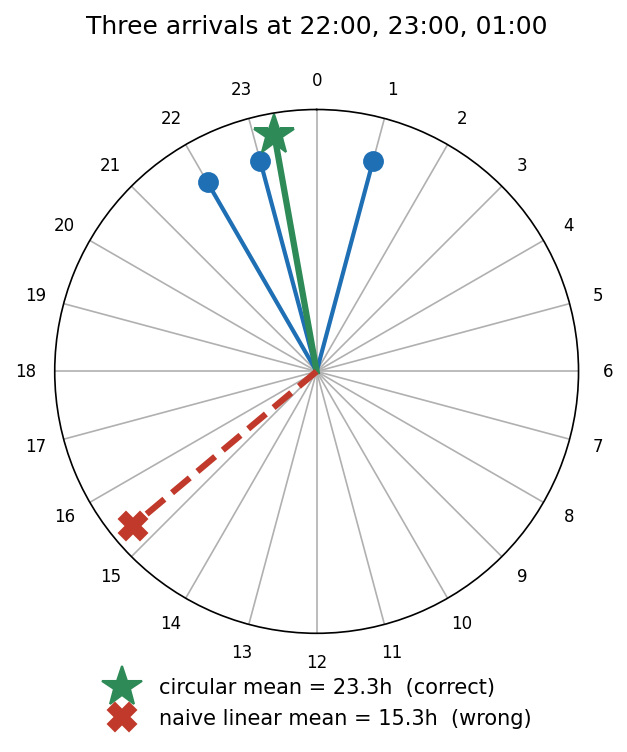
\includegraphics[width=0.62\textwidth]{figs/fig1_circular.png}
\caption{Why arrival hour needs a \emph{circular} mean. Three arrivals at 22:00, 23:00, 01:00 cluster near midnight. The circular mean (green star, 23.3\,h) sits inside the cluster; the naive linear mean (red X, 15.3\,h) lands on the opposite side of the clock --- completely wrong.}
\end{figure}

The fix is to treat each hour as an \textbf{angle}, average the unit vectors, and convert back:
\[
\theta_i=\frac{2\pi A_i}{24},\qquad
\bar A_u = \frac{24}{2\pi}\,\operatorname{atan2}\!\Big(\textstyle\sum_i\sin\theta_i,\ \sum_i\cos\theta_i\Big)\ (\mathrm{mod}\ 24).
\]
For the three arrivals $\{22,23,1\}$ this gives $\bar A_u=23.3$\,h (correct), versus the linear mean $15.3$\,h (wrong). Every per-user arrival summary in the benchmark uses this circular mean.

\subsection{Across-user standard deviation $\sigma_A,\sigma_D$ --- the heterogeneity signature}
Now the key quantity. We have one number per user (its $\bar A_u$, or its $\bar D_u$). The \textbf{across-user standard deviation} is the spread of \emph{those per-user numbers} across the whole fleet:
\[
\sigma_D=\operatorname{std}_u\big(\bar D_u\big),\qquad
\sigma_A=\text{(circular) std}_u\big(\bar A_u\big).
\]
It answers: \emph{``do different drivers actually behave differently?''}
\begin{itemize}[leftmargin=1.4em,itemsep=1pt]
\item \textbf{Large} $\sigma$ $\Rightarrow$ a diverse fleet: some drivers are morning commuters, others overnight chargers. This is property \textbf{P1 (per-user heterogeneity)}.
\item \textbf{Small} $\sigma$ $\Rightarrow$ everyone looks like the population average: a fleet of clones.
\end{itemize}
(For arrival we again use the \emph{circular} standard deviation, $\sigma_A=\frac{24}{2\pi}\sqrt{-2\ln \bar R}$, where $\bar R$ is the length of the mean unit vector of the per-user angles; the ruler-vs-clock caveat applies here too.)

\subsection{The pseudo-user trick: scoring baselines that have no users}
Here is the subtlety. The baselines emit an anonymous bag --- so how do we compute a \emph{per-user} statistic for them? We give them the fairest possible benefit of the doubt: we \textbf{split their pooled sessions into $K$ pseudo-users}, where $K$ and the per-user session counts match the real dataset, then compute $\sigma$ exactly as above. Averaging over many random splits removes luck.

Crucially, this isolates the effect of losing identity. Figure~\ref{fig:collapse} makes the point with the \emph{real} Norwegian sessions: we take the identical multiset of sessions and only change the \emph{assignment} of sessions to users.

\begin{figure}[h]
\centering
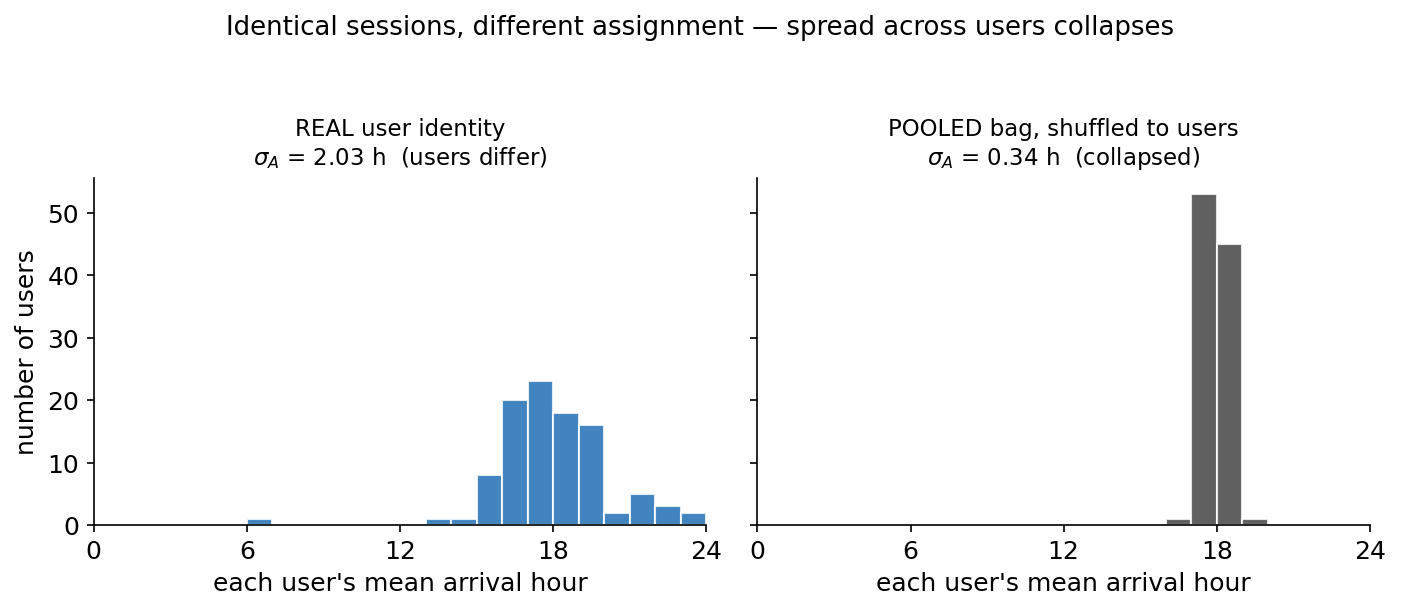
\includegraphics[width=0.92\textwidth]{figs/fig2_collapse.png}
\caption{The collapse, on real Norway data. \emph{Left}: with the true user labels, per-user mean arrival hours are spread out ($\sigma_A=2.03$\,h) --- a genuinely diverse fleet. \emph{Right}: the \emph{same sessions} randomly re-assigned to users (what a pooled generator implicitly assumes) pile every user's mean near the population average ($\sigma_A=0.34$\,h). Nothing about the marginals changed; only identity was destroyed.}
\label{fig:collapse}
\end{figure}

This is why marginal fidelity and heterogeneity are \emph{independent} tests. Figure~\ref{fig:structure} shows two fleets with an \textbf{identical aggregate marginal} but opposite internal composition.

\begin{figure}[h]
\centering
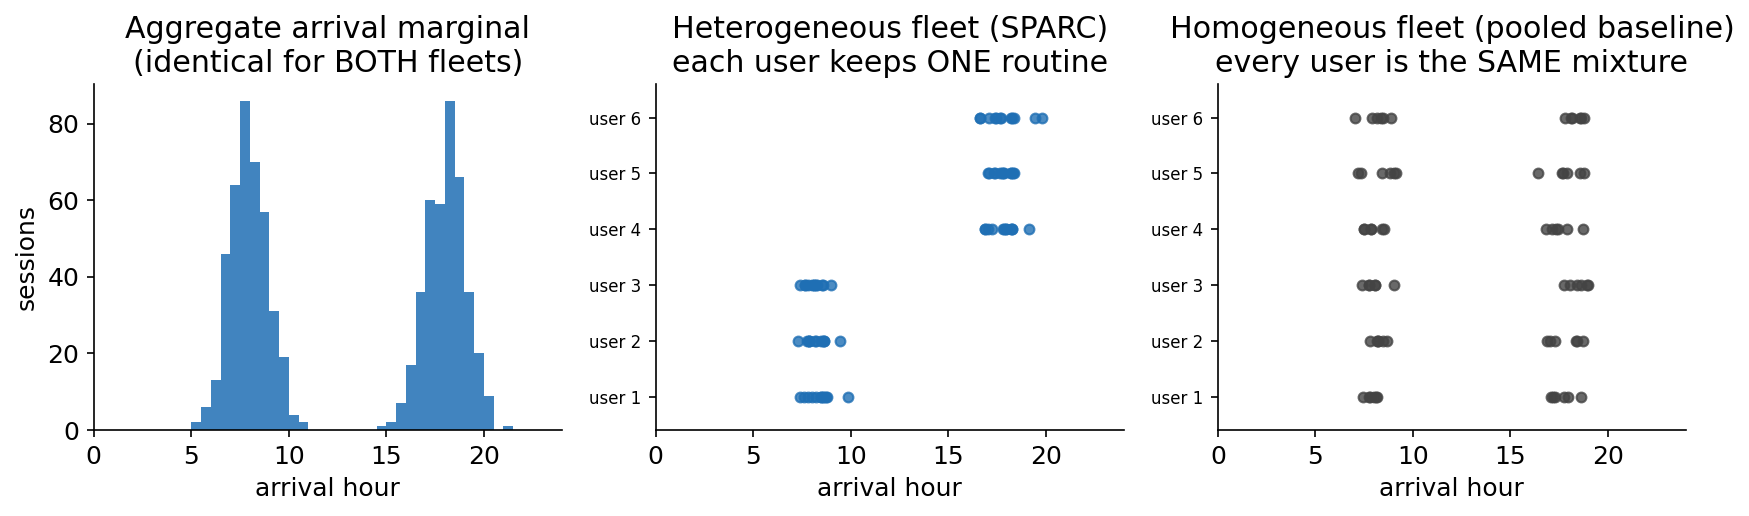
\includegraphics[width=0.98\textwidth]{figs/fig3_structure.png}
\caption{Same marginal, different structure. \emph{Left}: both fleets share the identical bimodal arrival histogram. \emph{Middle}: a heterogeneous fleet (SPARC) --- each user keeps one routine (some morning, some evening). \emph{Right}: a homogeneous fleet (pooled baseline) --- every user is the same morning+evening mixture. Only the per-user view distinguishes them.}
\label{fig:structure}
\end{figure}

\subsection{What Axis 2 shows}
SPARC reproduces the real across-user spread to within its seed variation on every dataset (e.g.\ Norway $\sigma_D=5.46\pm0.13$\,h against a real $5.66$\,h). The three pooled baselines collapse it three- to six-fold. They pass Axis~1 and fail Axis~2 --- they get the crowd right and every individual wrong.

\section{Axis 2b --- The joint load shape}
A second structural test that marginals cannot see is the fleet's \textbf{aggregate daily load profile}. Spreading each session's power $E_i/D_i$ over the clock hours it occupies gives
\[
L(h)=\sum_{i}\frac{E_i}{D_i}\,\big|[A_i,\,A_i+D_i]\cap[h,\,h+1]\big|,\qquad h=0,\dots,23 .
\]
This is a \emph{joint} functional: it depends on how $A$, $D$, and $E$ are \textbf{paired within a session}, not just on their separate histograms. Figure~\ref{fig:load} shows two session sets with \emph{identical} $A$, $D$, $E$ marginals but opposite $A$--$D$ pairings; their load curves are completely different. We score the normalised load shape with the same KL divergence, $\kl^{L}$. SPARC attains the lowest $\kl^{L}$ on all five datasets.

\begin{figure}[h]
\centering
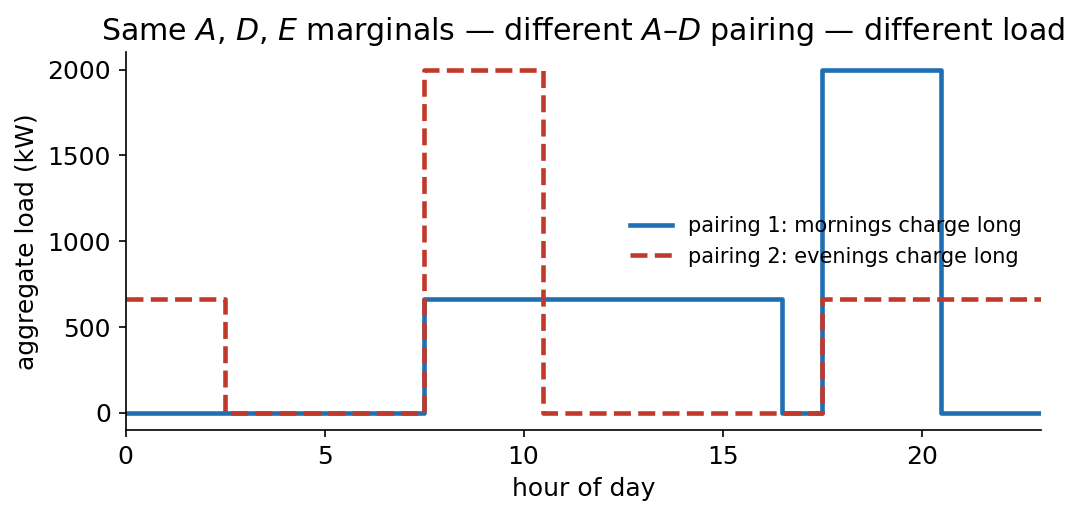
\includegraphics[width=0.72\textwidth]{figs/fig4_load.png}
\caption{The load is a joint quantity. Both populations have the same $A$, $D$, and $E$ marginals; they differ only in \emph{which} arrivals get the long durations. The resulting 24\,h load profiles peak at different times and heights --- so matching marginals does not guarantee matching grid impact.}
\label{fig:load}
\end{figure}

\section{Why the error bars (the seed sweep)}
A single run could be lucky. To show the results are stable we report \textbf{mean $\pm$ standard deviation}. For SPARC the spread is taken over \textbf{five independent simulation seeds}; for the baselines it is the estimator's own variability (bootstrap resampling for the KL scores, and the random pseudo-user partitions for $\sigma$). SPARC's seed spread is tiny (e.g.\ $\sigma_A$ std $\le0.13$\,h), and the gap to the baselines is many standard deviations wide --- so the separation is decisive, not noise.

\section{How to read the two benchmark tables}
\begin{table}[h]
\centering
\small
\begin{tabular}{@{}lll@{}}
\toprule
Symbol & Table & Plain-English meaning \\
\midrule
$A,D,E$ (KL) & marginals & how far each overall histogram is from real (lower better) \\
$\sigma_A$ & structure & spread of per-user \emph{arrival} routines (closer to Real better) \\
$\sigma_D$ & structure & spread of per-user \emph{durations} (closer to Real better) \\
$\kl^{L}$ & structure & error in the 24\,h fleet load shape (lower better) \\
\bottomrule
\end{tabular}
\end{table}

The two tables are meant to be read \emph{together}. The marginal table asks ``does the crowd look right?'' and the copula wins it. The structure table asks ``does each driver look right, and does the fleet load come out right?'' and only SPARC matches reality. Matching marginals is necessary but not sufficient: a generator can be marginally perfect yet produce a fleet of identical users, misrepresenting exactly the between-user diversity that drives coincident peak demand, transformer sizing, and managed-charging headroom.

\paragraph{One-line takeaway.} SPARC is the only method that simultaneously matches the marginals (Axis~1), the per-user heterogeneity (Axis~2), and the joint load shape (Axis~2b) --- and it does so from only tens of sessions per user, without per-context tuning.

\end{document}
